\chapter{Materiais e Métodos}
\label{cap:03}

Para a prototipagem do traçador I-V houve a necessidade de se seguir as seguintes etapas:
\begin{itemize}
	\item Integração entre os componentes do protótipo sendo eles:
	\begin{itemize} 
		\item Arduino;
		\item Carga eletrônica;
		\item Painel solar;
		\item Sensor ADS1115;
		\item Cartão SD.
	\end{itemize}
	\item Teste de precisão na coleta de dados;
	\item Padronização e fixação do ambiente de testes;
	\item Teste de do protótipo;
	\item Armazenamento da amostragem coletada;
	\item Análise e tratamento da amostra;
	\item Verificação e resolução de erros e/ou problemas.

\end{itemize}

\subsection{Arduino}
A plataforma Arduino foi utilizada de maneira centralizar o controle de todos os periféricos necessários para a prototipagem. Foi utilizado as saídas PWM, Barramento I2C e SPI.

IMAGEM que será adicionada
%Imagem ARduino+I2C+SPI

\subsection{I2C e SPI}
As comunicações I2C e SPI permitiram o uso de ferramentas não disponíveis no hardware original do Arduino, como a utilização de um ADC de 16bits ou do cartão SD para armazenamento dos dados.

Imagem SDCARDMOD

\subsection{Carga Eletronica}
A carga eletrônica permitiu a variação dos valores de corrente e tensão do painel, fator indispensável para a ação do traçador.

Imagem Carga eletrônica

\subsection{Circuito Completo}

Se observa na figura~\ref{label} como se assemelha o circuito completo do traçador de curvas I-V.

\subsection{Métodos}
\subsubsection{Controle de Variáveis}
Durante os experimentos foram necessários atestar alguns aspectos, garantindo maior estabilidade no processo de aquisição de dados:
\begin{itemize}
\item Irradiância solar fixa;
\item Uso de sensores Precisos
\end{itemize}

Para garantir maior veracidade e precisão na coleta de dados, foi realizado um teste com diferentes valores a serem coletados pelo sensor utilizando o ADS1115 e um multímetro de alta precisão, ao se comparar os dados do multímetro e do ADS1115, nota-se a os valores contíguos do sensor em relação ao multímetro, como observável na figura~\ref{fig:Precisao}.

\FloatBarrier
\begin{figure}[!htbp]
	\centering
	%scale redimensiona a figura.
	%1.5 = 150% do tamanho original
	%1 = 100% do tamanho original
	%0.20 = 20% do tamanho original
	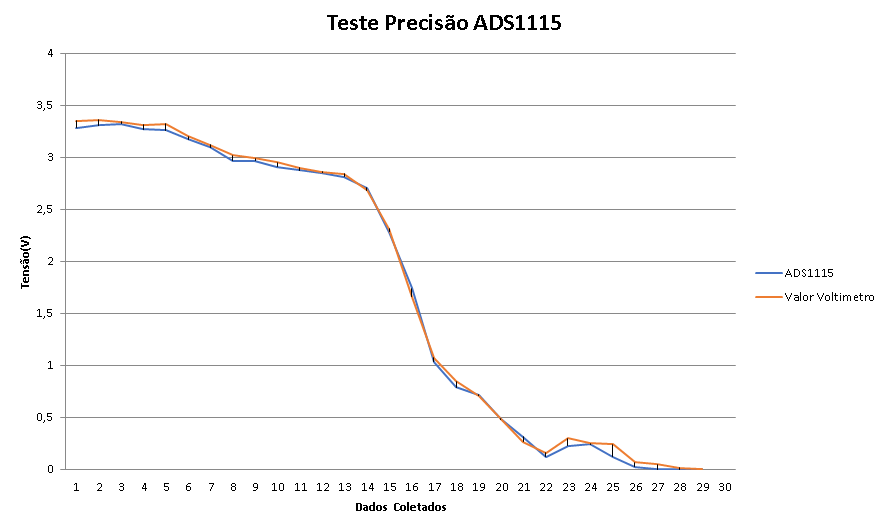
\includegraphics[scale=0.6]{imagens/Precisao}
	\caption{Diferentes valores de tensão e comparação entre o sensor e um multímetro comercial. Fonte: Elaborado pelo Autor. %Disponível em %<https://www.sdcard.org/developers/overview/family/index.html>.}
	}
	\label{fig:Precisao}
\end{figure}
\FloatBarrier

Considerando o clima e tempo instável oscilando entre dias chuvosos, nublados e alguns ensolarados, houve a necessidade de uma maneira de viabilizar os testes ainda que houvesse clima desfavorável. O engenho que permitiu tal feito foi o uso de uma lampada halogênea, que teve como papel gerar e simular a mesma irradiância que seria gerada pelo Sol em um dia sem nuvens.  

Imagem Da Lampada
...

\subsubsection{Comportamento do Protótipo}

De maneira a torna o uso do traçador mais acessível e funcional, foram instalados LEDs que apresentam em qual parte do processo de aquisição de dados o traçador se encontra, e um LED para sinalização de erros durante a aquisição de dados, sendo suas cores:

\begin{itemize}
	\item Amarelo;
	\item Branco;
	\item Verde 1;
	\item Verde 2;
	\item Vermelho.
\end{itemize}

Foram utilizadas diferentes combinações de LEDs para sinalizar as diferentes etapas, assim como  reproduzido na tabela~\ref{tab:LEDS}.

\FloatBarrier
\begin{table}[!htbp]
	\centering
	\caption{Combinação dos LEDs de sinalização}
	\begin{tabular}{ c | c }
		\hline
		\textbf{Combinações de Cores} & \textbf{Função}                                   \\ \hline
		Vermelho                      & Erro durante a coleta                             \\ \hline
		Amarelo,Verde1                & Aguardando habilitação pelo usuário para a coleta \\ \hline
		Verde2                        & Coleta de dados habilitada                        \\ \hline
		Branco                        & Coletando de dados                                \\ \hline
		Branco,Verde1,Vermelho        & Finalização da coleta                             \\ \hline
	\end{tabular}
	\\ \vspace{0.2cm}
	\textbf{Fonte:} Elaborada pelo autor
	\label{tab:LEDS}
\end{table}
\FloatBarrier




